
This section is built on our code repository, which is available at \textcolor{red}{\url{GITHUB}}.
\noteAnt{a compléter}
All the competitive methods are implemented in C, using arbitrary precision arithmetic
and a flow of cryptographic random bits. A part of the implementation is devoted to reproduce our experimental results.
Experiments were conducted on a MacBook Pro (Apple M4 Pro chip, 14-core CPU) with 48GB of unified memory.
%, running macOS 26.6.2.


\subsection{Overview of the experimental approach}

This section evaluates the practical performance of the algorithms introduced in \Cref{sec:algo}
with a focus on measurable scalability limits, targeting five quantities: preprocessing time, sampling
throughput, memory footprint, random-bit consumption, and savings. All computations use exact integer
arithmetic, so results are free of floating-point rounding artifacts, and rely on compact data structures
that make explicit the core trade-off between entropic efficiency (in bits) and time efficiency.

A distinctive feature of our implementation is native support for arbitrary-precision arithmetic 
(to the best of our knowledge, the only one in our comparison to provide exact sampling at arbitrary
precision). Sampling draws from a background thread that continuously refills a bitstream, enabling the use
of expensive cryptographic random bits with a limited impact on performance, since bit
production is decoupled from and overlapped with sampling (reported times include its CPU time).



\subsection{Case Study: Combinatorial Chemistry}
\label{sec:chemie}

What is following illustrates how exact sampling becomes essential
when the underlying combinatorial space is too large, as in several nowadays applications.
The chemical space, i.e. the set of all combinatorially plausible stable
molecules, is far too vast to be enumerated. Reference databases report
sizes ranging from $9.7 \cdot 10^{7}$ molecules for the smallest
structures (e.g., GDB-17, up to 17 heavy atoms) to several trillion
compounds for modern make-on-demand combinatorial
libraries~\cite{SSHL26}, and beyond roughly thirty heavy atoms the
number of possible structures far exceeds $2^{64} \approx 1.8 \cdot
10^{19}$. Consequently, any statistical analysis based on a subset of this
space is structurally biased unless the sample is representative of the
true underlying distribution.

To address this context, Monterrubio-Chanca and von Rudorff~\cite{MR25}
proposed a method for producing unbiased, representative samples of
chemical space without ever enumerating it, applicable to molecules containing
on the order of 30 heavy atoms. Obviously, this is a regime in which exhaustive enumeration is
impossible. The method proceeds in five steps:
\begin{enumerate}
  \item Generation of all theoretically possible chemical formulas by
    integer partitioning; %, from valence and stoichiometry constraints;
  \item Grouping of these formulas by degree sequence;
    %, the combinatorial skeleton of the molecular graph, independent of the specific chemical elements involved;
  \item Distinction between ``pure'' and ``non-pure'' sequences, depending
    on whether several elements of the same valence appear;
  \item Estimation of the size of each group, either through exact
    counting or through a heuristic based on the graph's average path length when
    exact counting proves too costly;
  \item Weighted random sampling among the groups, proportional to their
    estimated size, followed by the sampling of a representative molecule
    within the chosen group.
\end{enumerate}
We note that the two steps \textbf{1.} and \textbf{5.} are classical in the context of combinatorics and combinatorial
algorithm design. Especially step \textbf{5.} is a classical application of the Alias method.
All their results are reproducible through their open-source \texttt{nablachem} Python
package~\cite{nablachem}.

Using their library, we derive the distribution of chemical molecules containing 32 heavy atoms, among Carbon, Hydrogen, Oxygen, Nitrogen, and Fluorine. The total number of molecules is $n = 20\,484$, and the sum of their weights is about $1.25 \cdot 2^{168} \approx 4.7 \cdot 10^{50}$. Thus in the following benchmarks for the sampling method, we used these parameters, which seem representative of the actual combinatorial chemistry research. Remark that step \textbf{5.} cannot be performed without bias in their Python library based on floating-point arithmetic samplers that are not precise enough in this regime. Note that exactness is
understood with respect to the supplied weights: when some group sizes are only estimated heuristically
(step \textbf{4.}), our sampler reproduces this estimated distribution exactly, but does not correct the
estimation itself. More details about this case study case be found in our code repository.
%Appendix~\ref{app:chemistry}.


\subsection{Algorithms with arbitrary precision integers}


Following the design of our Integer-Alias Sampler, the next phase focuses on an experimental evaluation of our algorithm against existing methods (adapted with arbitrary precision). We start from the code repository of Saad et al.~\cite{SFRM19} in order to add our implementation in their comparison: we thus are able to run all their benchmarks. We have adapted the original memory consumption analysis to the precise size used by the data structures built by the preprocessing step.

% \noteAnt{Dire un mot qu'on a prog en C, avec GMP et que les exp sont faite sur la spec de ma machine,
% dire qu'on a modifié l'analyse de l'espace mémoire que nous ne trouvions pas adéquat pour la comparaison entre preprocessing, qu'on gère une pile d'alea pour se baser sur de l'alea crypto sans ralentir la construction de la simulation}

 While Saad et al. compared many literature approaches to emphasize random bit consumption, we retain the three most relevant ones for our constraints (time, memory, and random bits) at arbitrary precision, all exact (floating-point samplers are left out: on 179 of our 201 distributions, they would never draw some objects, whose bucket share $n w_i/w$ is below $2^{-53}$):
\begin{itemize}
    \item \textsc{Fldr} Sampler: Saad et al.~\cite{SFRM19} that we adapted for arbitrary-precision integers;
    \item \textsc{Aldr} Sampler: Draper and Saad~\cite{DS26}, an improvement of FLDR in the context of random bit consumption, that we also adapted for arbitrary-precision integers;
    \item Rust-Alias Sampler: Rust Developers, a variant of Walker version coded in Rust with integer arithmetic~\cite{Rust25}, where we also have modified types to support arbitrary-precision integers;
    \item Fraction-Alias Sampler: our new exact version of Walker-Alias using exact rational fractions (with arbitrary precision) instead of floating-point numbers;
    \item our Integer-Alias Sampler: our new algorithmic approach, in two implementations of the same table: \emph{v1} saves random bits with Lumbroso's optimal \textsc{Uniform} and \textsc{Bernoulli}~\cite{Lumbroso13}; \emph{v2} saves time with Lemire's \textsc{Uniform}~\cite{Lemire19} and a Bernoulli test on the same 64-bit word (64 bits per draw).
\end{itemize}

The experimental protocol starts by fixing the distribution size (the number of objects), that
we take to be $n = 20\,484$ and the total weight distribution to be the one computed in the context of combinatorial chemistry (see Section~\ref{sec:chemie}) $w \approx 4.7 \cdot 10^{50}$.
The measurements were collected on a set of random distributions following a Dirichlet distribution.
Using a Dirichlet distribution allows varying the entropy while maintaining fixed values for parameters $n$ and $w$. The distribution itself is not of major importance, once we can choose for the average weight of an object or the entropy of the resulting random distribution (e.g. a gaussian distribution of weights would have given the same kind of experimental simulations).
The observed entropy corresponds to Shannon entropy. The latter is a central theoretical measure
in the context of random sampling. We refer the reader to the seminal paper of
Knuth and Yao~\cite{KY76} for a general overview. Essentially, we note that the closer a distribution is to a uniform distribution, the higher its entropy (bounded by $\log_2(n)$).
Conversely, a strongly biased distribution (e.g., one element with a very large weight and many elements with a weight of $1$) results in lower entropy.
For each distribution, among the 200 random ones, 10 millions of objects have been sampled to measure the average sampling time and the average number of random bits consumed.

\begin{figure}[htb]
    \centering
    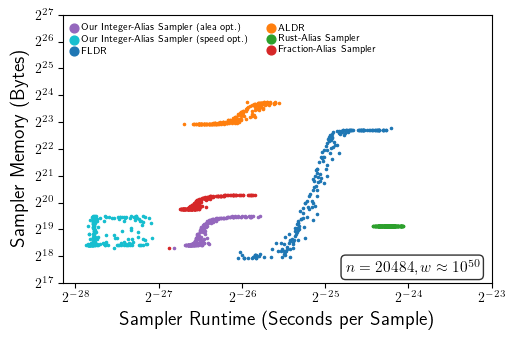
\includegraphics[width=0.47\textwidth]{figs/Runtime-memory.png}
    \hfill
    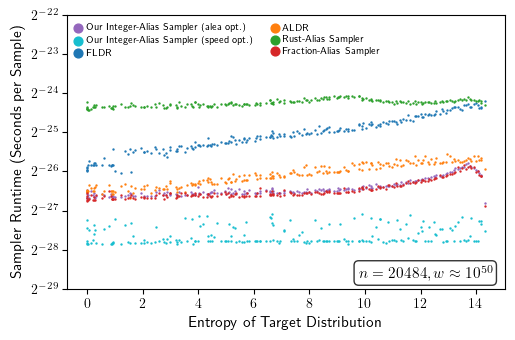
\includegraphics[width=0.47\textwidth]{figs/Entropy-runtime.png}
    \caption{Sampling runtime under arbitrary precision, against the memory footprint (left) and the entropy of the distributions (right).}
    \label{fig:runtime_memory}
\end{figure}

Figure~\ref{fig:runtime_memory} (left) plots the runtime of the sampling step against the memory footprint of the internal data structures, one dot per random distribution (averaged over 10 million samples; $2^{-20}\text{s} = 0.95\,\mu\text{s}$ and $2^{20}\text{B} = 1\text{MB}$). The tight horizontal clustering of Alias-based methods reflects their $O(1)$ sampling step, structurally independent of the distribution, whereas \textsc{Fldr} and \textsc{Aldr} spread much more widely, exposing their sensitivity to its shape. The picture traces an implicit Pareto frontier: \textsc{Fldr} and \textsc{Aldr} are fast but memory-intensive on favorable distributions, while Alias-based approaches remain compact and predictable. Within this family, our Integer-Alias Sampler consistently runs faster than Rust-Alias at comparable memory cost, since normalizing by $\mathtt{cs}$ rather than by the full cumulative weight $w$ speeds up the sampling step regardless of the distribution; v2 is the fastest of all, $2.3$ times faster than v1.

\begin{figure}[ht]
    \centering
    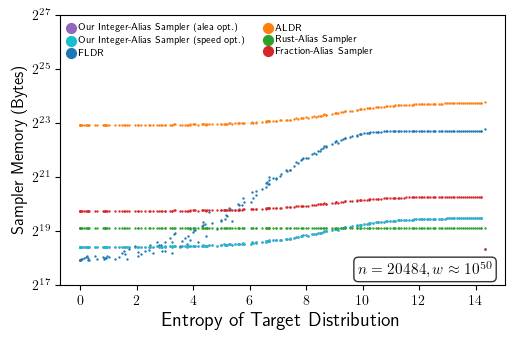
\includegraphics[width=0.38\textwidth]{figs/Entropy-memory.png}
    \hfill
    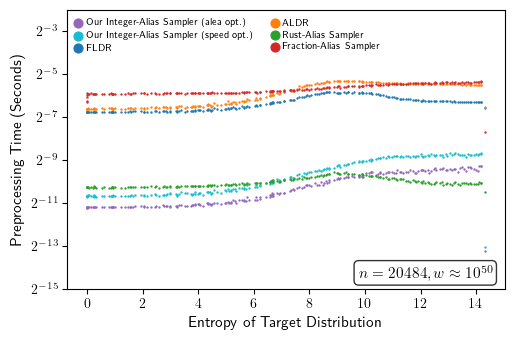
\includegraphics[width=0.38\textwidth]{figs/Entropy-preprocessing.png}\\[0.3em]
    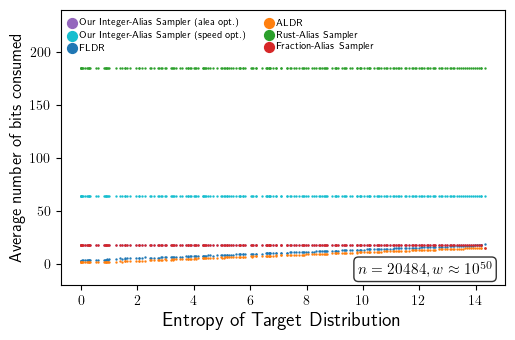
\includegraphics[width=0.38\textwidth]{figs/Entropy-bits.png}
    \hfill
    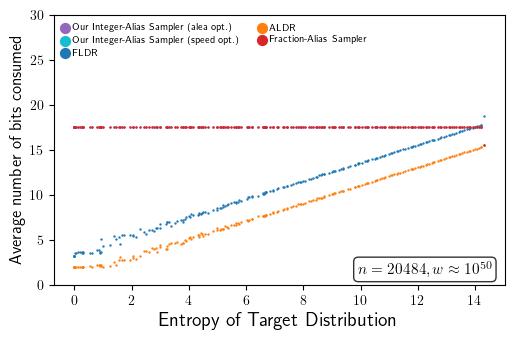
\includegraphics[width=0.38\textwidth]{figs/Entropy-bits2.png}
    \caption{Memory footprint (top left), preprocessing time (top right), and randomness consumption (bottom) of the compared algorithms under arbitrary precision, against the entropy. The bottom-right plot zooms into the bottom-left one (capped at 30 bits).}
    \label{fig:entropy_all}
\end{figure}

Figure~\ref{fig:runtime_memory} (right) confirms that Alias-based runtimes stay near-constant across the entropy spectrum: the preprocessing step encodes the whole distribution into the table, so each draw only needs a uniform bucket selection and a single Bernoulli test. \textsc{Fldr} and \textsc{Aldr}, built on the DDG-tree framework of Knuth and Yao~\cite{KY76}, instead consume random bits one at a time to navigate a binary decision tree whose expected depth equals the distribution's Shannon entropy; they are therefore \emph{faster} at low entropy (skewed distributions yield short, predictable tree paths) and \emph{slower} as entropy approaches $\log_2(n)$ (near-uniform distributions require paths of maximal depth). The crossover, at roughly half the maximum entropy, marks the point where \textsc{Aldr}'s entropy-proportional cost exceeds the constant cost of our sampler. The combinatorial-chemistry case study of \Cref{sec:chemie}, being strongly skewed, falls in the low-entropy regime most favorable to \textsc{Fldr} and \textsc{Aldr}; even there, our Integer-Alias Sampler stays within the same order of magnitude in runtime while using strictly less memory.

Regarding memory (Figure~\ref{fig:entropy_all}, top left), Alias-based approaches are more compact than \textsc{Aldr} across all entropies, and than \textsc{Fldr} except at low entropy, where its tree is small (we report the exact footprint of the preprocessed data structure). Within the Alias family, although Rust-Alias's integer weights are $n$ times larger than ours (it normalizes by the total weight $w$ rather than by $\mathtt{cs}$), our table needs at most one extra cell (since $\cs\leq n-1$), so both approaches use similar memory. This confirms that the runtime gap seen in Figure~\ref{fig:runtime_memory} (left) comes from the arithmetic cost of the Bernoulli step on large integers, not from memory layout. The Fraction-Alias Sampler's table, in contrast, is about twice as large, since it stores a full rational number (numerator and denominator) per entry instead of a single integer.

Figure~\ref{fig:entropy_all} (top right) shows the preprocessing time (file parsing excluded; the Python construction of \textsc{Fldr}~\cite{SFRM19} is replaced by an equivalent C port): ours and Rust-Alias's stay below $2.5$\,ms, twenty times less than \textsc{Fldr}, \textsc{Aldr} (scanning each weight at every tree level) and Fraction-Alias.

Figure~\ref{fig:entropy_all} (bottom row) reports the average number of random bits consumed per sample, excluding (bottom right) Rust-Alias, whose consumption is an order of magnitude higher, and v2. This is structural: Rust-Alias draws a uniform integer in $[0, w)$, costing $\log_2(w) \approx 153$ bits, instead of a Bernoulli test costing only $\log_2(n) \approx 14$ bits as in our sampler --- the direct price of skipping weight normalization, which makes that approach impractical at large precision regardless of its time efficiency.

Among the remaining algorithms, \textsc{Fldr} and \textsc{Aldr} consume fewer random bits than our sampler, with \textsc{Fldr} reaching the information-theoretic optimum of Knuth and Yao~\cite{KY76}; however this advantage narrows as entropy grows, since the dominant cost then becomes the uniform bucket selection ($\log_2(n)$ bits for every algorithm). Near the uniform distribution, this fixed cost dominates and our overhead relative to the optimum becomes negligible: in that regime, our sampler simultaneously achieves $O(1)$ sampling time, a memory footprint among the smallest of the compared methods, and near-optimal bit consumption.
